\documentclass{article}

\usepackage[utf8]{inputenc}
\usepackage[T1]{fontenc}
\usepackage{graphicx}
\usepackage{listings}

\begin{document}

\begin{flushright}
Błażej Pawluk, 279738
\end{flushright}

% Tytuł sprawozdania
\title{WSI, Laboratorium, Lista 1}
\date{}
\maketitle

\section*{Pobranie danych ze zbioru EMNIST MNIST}
\begin{lstlisting}[language=Python, frame=single, breaklines=true, breakatwhitespace=true]
from tensorflow.keras.datasets import mnist

(x_train, y_train), (x_test, y_test) = mnist.load_data()

x_train = x_train.astype('float32') / 255.0
x_train = x_train.reshape(x_train.shape[0], -1)

x_test = x_test.astype('float32') / 255.0
x_test = x_test.reshape(x_test.shape[0], -1)

y_train = to_categorical(y_train, num_classes)
y_test = to_categorical(y_test, num_classes)
\end{lstlisting}

\begin{figure}[h!]
	\centering
	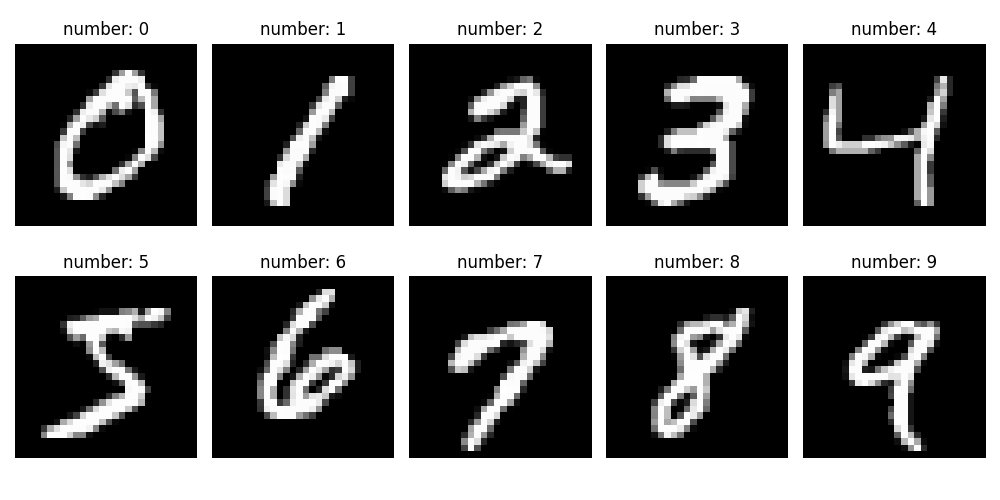
\includegraphics[width=1\textwidth]{images/numbers.png}
	\caption{Cyfry ze zbioru EMNIST MNIST, na których sieć jest trenowana}
\end{figure}

\section*{Tworzenie i kompilacja modelu}
\begin{lstlisting}[language=Python, frame=single, breaklines=true, breakatwhitespace=true]
# tworzenie modelu
model = Sequential()
model.add(Dense(units=128, input_shape=(784,), activation='relu'))
model.add(Dense(units=128, activation='relu'))
model.add(Dropout(0.25))
model.add(Dense(units=num_classes, activation='softmax'))

# kompilacja modelu
model.compile(
	loss='categorical_crossentropy',
	optimizer='adam',
	metrics=['acc', 'precision', 'recall']
)
model.summary()
\end{lstlisting}

\begin{figure}[h!]
	\centering
	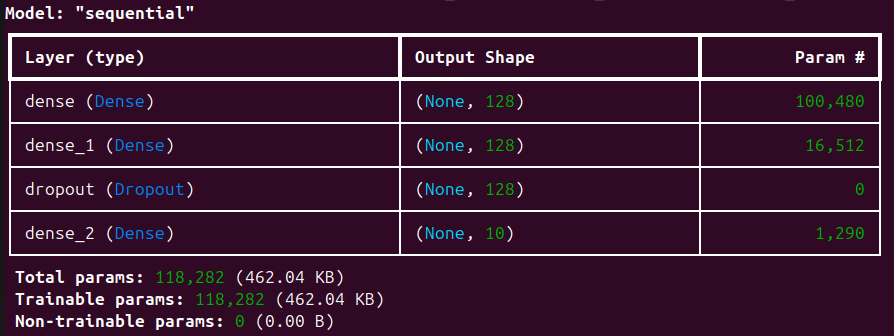
\includegraphics[width=1\textwidth]{images/model.png}
	\caption{Schemat sieci, pokazany dzięki model.summary()}
\end{figure}

\section*{Trenowanie modelu i statystyki z treningu}
\begin{lstlisting}[language=Python, frame=single, breaklines=true, breakatwhitespace=true]
# trenowanie modelu
train = model.fit(
	x=x_train, 
	y=y_train, 
	batch_size=512, 
	epochs=10
)

# wyświetlenie statystyk treningu
acc = train.history['acc']
loss = train.history['loss']
precision = train.history['precision']
recall = train.history['recall']

fig, ax1 = plt.subplots()
ax2 = ax1.twinx()

ax1.set_xlabel('epoka')
ax1.set_ylabel('accuracy / precision / recall')
ax2.set_ylabel('loss')

ax1.plot(range(1, len(acc) + 1), acc, label='accuracy')
ax1.plot(range(1, len(precision) + 1), precision, label='precision')
ax1.plot(range(1, len(recall) + 1), recall, label='recall')
ax2.plot(range(1, len(loss) + 1), loss, label='loss')

fig.legend()
plt.title('training statistics')
plt.tight_layout()
plt.show()
\end{lstlisting}

\begin{figure}[h!]
	\centering
	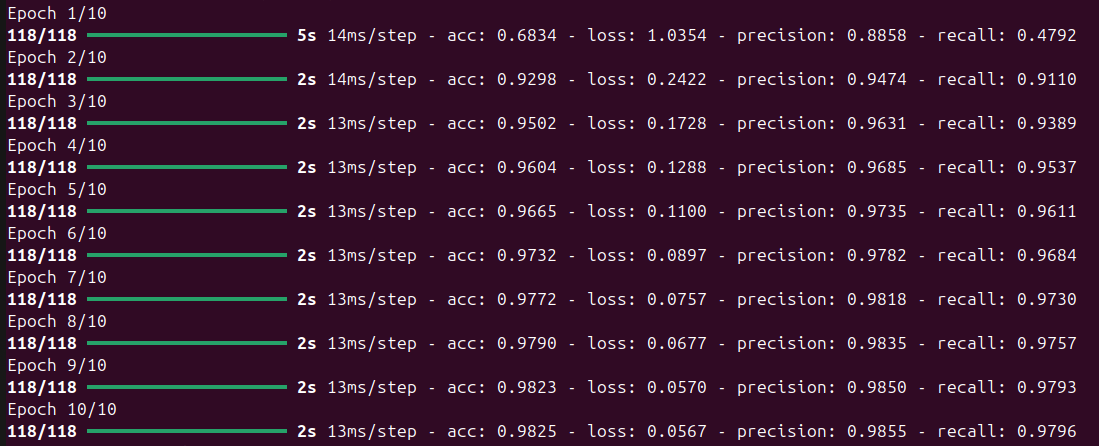
\includegraphics[width=1\textwidth]{images/training.png}
	\caption{Kolejne epoki i ich statystyki}
\end{figure}

\begin{figure}[h!]
	\centering
	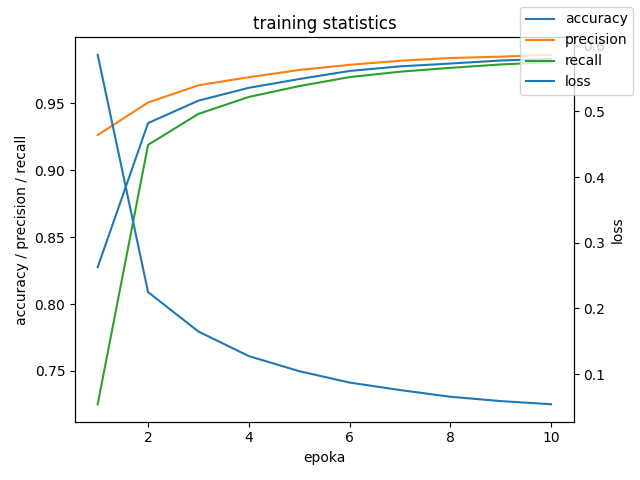
\includegraphics[width=1\textwidth]{images/training_stats.png}
	\caption{Statystyki: accuracy, precision, recall, loss, w treningu sieci neuronowej}
\end{figure}

\section*{Testy na zbiorze MNIST}
\begin{lstlisting}[language=Python, frame=single, breaklines=true, breakatwhitespace=true]
# testowanie na zbiorze MNIST
print("testing on MNIST dataset:")
loss, acc, precision, recall = model.evaluate(x_test, y_test)

print(f"accuracy: {acc*100:.2f}%")
print(f"loss: {loss*100:.2f}%")
print(f"precision: {precision*100:.2f}%")
print(f"recall: {recall*100:.2f}%")

y_pred_prob = model.predict(x_test)
y_pred = np.argmax(y_pred_prob, axis=1)
y_real = np.argmax(y_test, axis=1)
conf_matrix = confusion_matrix(y_real, y_pred)

fig, ax = plt.subplots(figsize=(15, 10))
ax = sb.heatmap(conf_matrix, annot=True, fmt='d', ax=ax)
ax.set_xlabel('prediction')
ax.set_ylabel('real')
ax.set_title('confusion matrix (testing on MNIST dataset)')

plt.tight_layout()
plt.show()
\end{lstlisting}

\begin{figure}[h!]
	\centering
	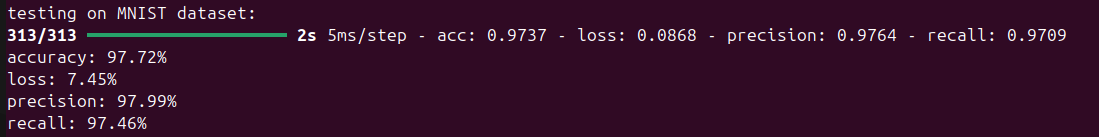
\includegraphics[width=1\textwidth]{images/mnist_test_stats.png}
	\caption{Statystyki: accuracy, precision, recall, loss, w teście na zbiorze EMNIST MNIST}
\end{figure}

\begin{figure}[h!]
	\centering
	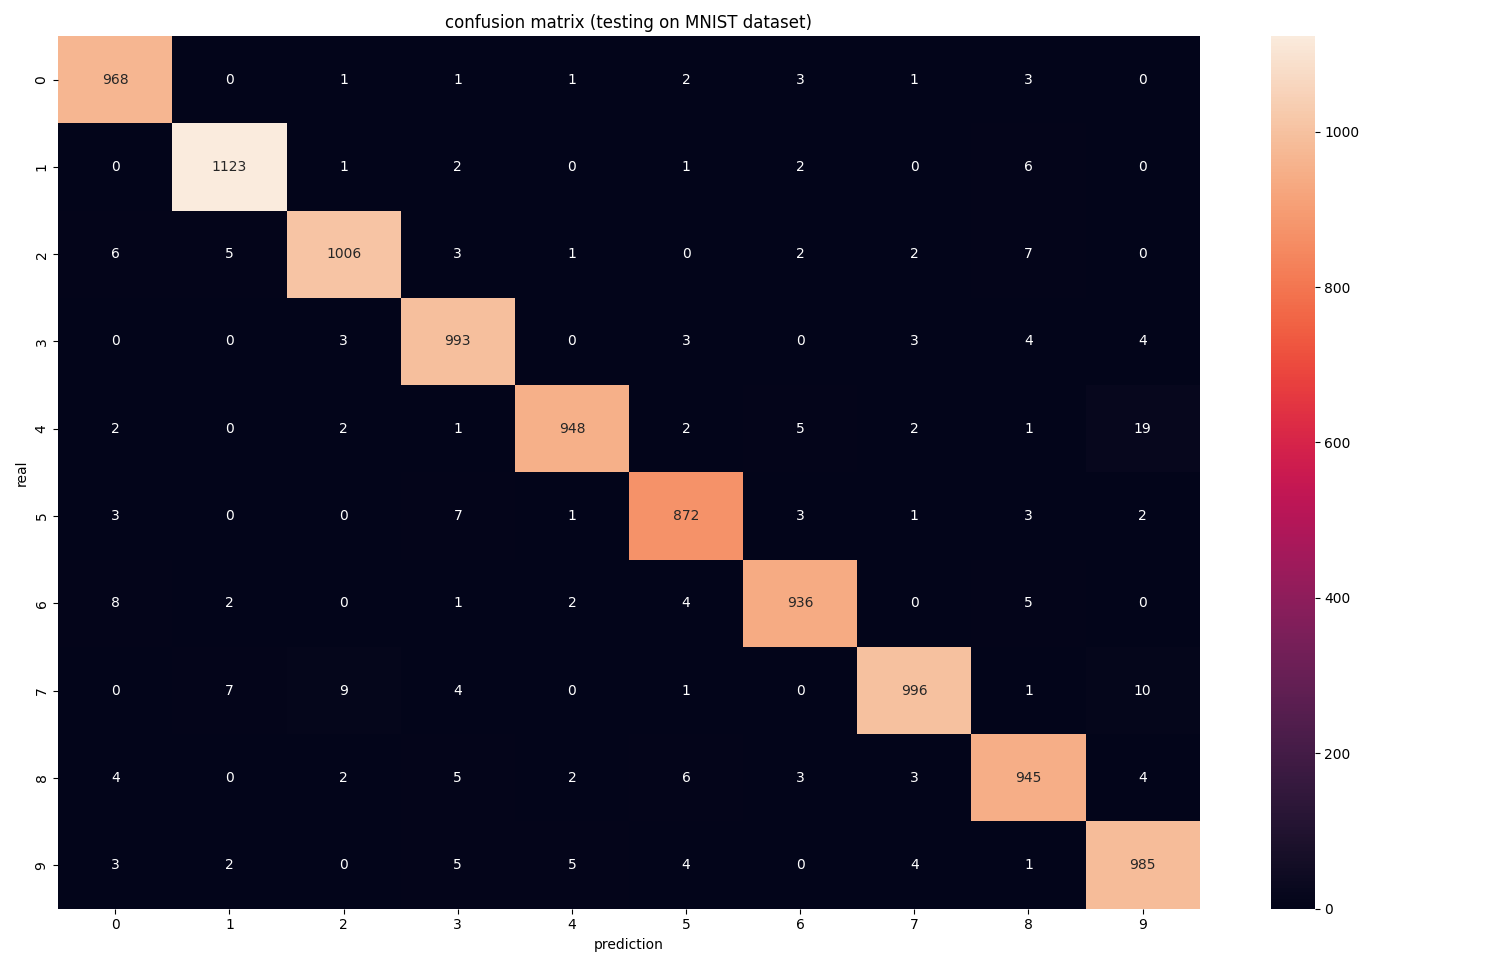
\includegraphics[width=1\textwidth]{images/mnist_conf_matrix.png}
	\caption{Confusion matrix dla testów na zbiorze EMNIST MNIST}
\end{figure}

\section*{Import własnego zbioru testowego}
\begin{lstlisting}[language=Python, frame=single, breaklines=true, breakatwhitespace=true]
x_my = np.empty([30, 28, 28])
y_my = np.array([i for i in range(num_classes) for _ in range(3)])

i = 0
for digit in range (0, num_classes):
	for number in range(1, 4):
		image = Image.open(f"myDigits/{digit}-{number}.png").convert('L')
		image = image.resize((28, 28))
		x_my[i] = np.array(image)
		i += 1

x_my /= 255.0
x_my = x_my.reshape(x_my.shape[0], -1)

y_my = to_categorical(y_my, num_classes)
\end{lstlisting}

\begin{figure}[h!]
	\centering
	
\includegraphics[width=1\textwidth]{images/test_number.png}
	\caption{Przykładowa cyfra z mojego zbioru testowego}
\end{figure}

\section*{Testy na własnym zbiorze testowym}
\begin{lstlisting}[language=Python, frame=single, breaklines=true, breakatwhitespace=true]
# testowanie na własnym zbiorze
print("testing on my dataset:")
loss, acc, precision, recall = model.evaluate(x_my, y_my)

print(f"accuracy: {acc*100:.2f}%")
print(f"loss: {loss*100:.2f}%")
print(f"precision: {precision*100:.2f}%")
print(f"recall: {recall*100:.2f}%")

y_pred_prob = model.predict(x_my)
y_pred = np.argmax(y_pred_prob, axis=1)
y_real = np.argmax(y_my, axis=1)
conf_matrix = confusion_matrix(y_real, y_pred)

fig, ax = plt.subplots(figsize=(15, 10))
ax = sb.heatmap(conf_matrix, annot=True, fmt='d', ax=ax)
ax.set_xlabel('prediction')
ax.set_ylabel('real')
ax.set_title('confusion matrix (testing on my dataset)')

plt.tight_layout()
plt.show()
\end{lstlisting}

\begin{figure}[h!]
	\centering
	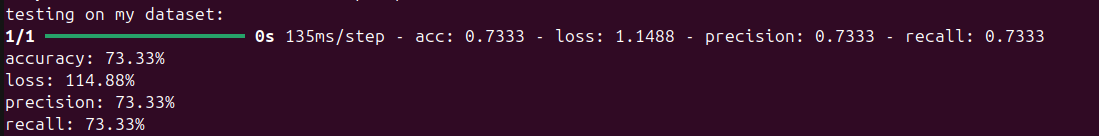
\includegraphics[width=1\textwidth]{images/my_test_stats.png}
	\caption{Statystyki: accuracy, precision, recall, loss, w teście na moim zbiorze}
\end{figure}

\begin{figure}[h!]
	\centering
	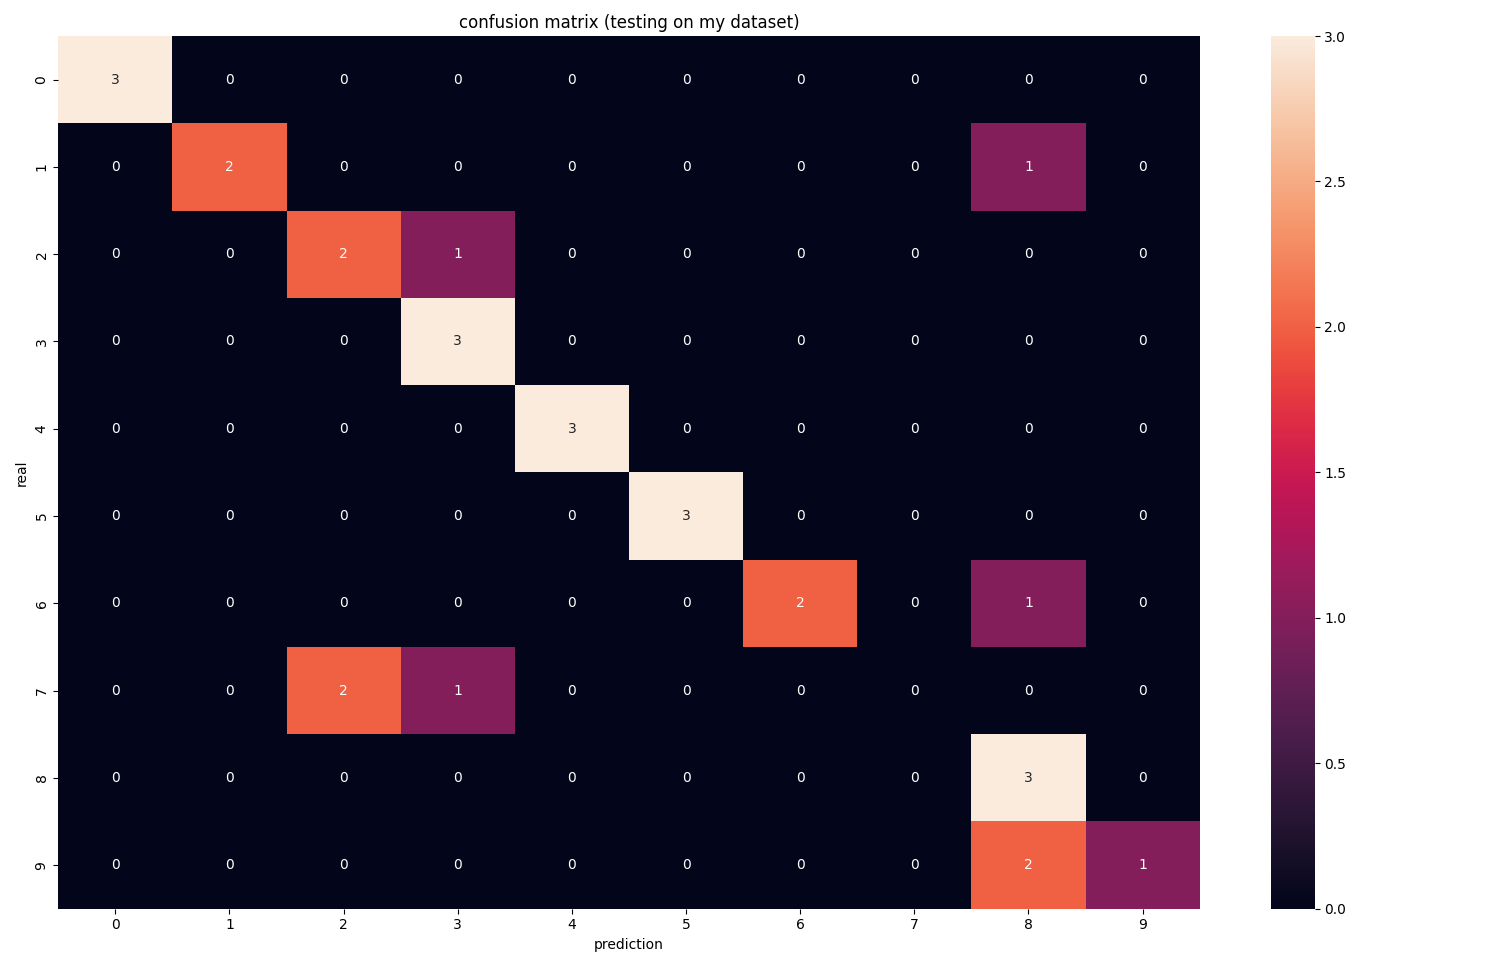
\includegraphics[width=1\textwidth]{images/my_conf_matrix.png}
	\caption{Confusion matrix dla testów na moim zbiorze}
\end{figure}

Wnioski: Z moim zbiorem testowym sieć poradziła sobie gorzej niż ze zbiorem EMNIST MNIST (73.33\% vs 97.72\%). Może to być spowodowane różnicą w sposobie pisania cyfr, np. dla cyfry 7 pisanej bez kreski w zbiorze EMNIST MNIST, albo 9 z prostą kreską pionową zamiast zaokrąglonej.

\section*{Tworzenie i trenowanie Random Forest}
\begin{lstlisting}[language=Python, frame=single, breaklines=true, breakatwhitespace=true]
# tworzenie modelu
model = RandomForestClassifier(n_estimators=10, random_state=42)

# trenowanie modelu
model.fit(x_train, y_train)
\end{lstlisting}

\section*{Testowanie Random Forest na zbiorze EMNIST MNIST}
\begin{lstlisting}[language=Python, frame=single, breaklines=true, breakatwhitespace=true]
# testowanie na zbiorze MNIST
print("testing on MNIST dataset:")
y_pred_prob = model.predict(x_test)

acc = accuracy_score(y_test, y_pred_prob)
precision = precision_score(y_test, y_pred_prob, average='macro')
recall = recall_score(y_test, y_pred_prob, average='macro')

print(f"accuracy: {acc*100:.2f}%")
print(f"precision: {precision*100:.2f}%")
print(f"recall: {recall*100:.2f}%")

y_pred = np.argmax(y_pred_prob, axis=1)
y_real = np.argmax(y_test, axis=1)
conf_matrix = confusion_matrix(y_real, y_pred)

fig, ax = plt.subplots(figsize=(15, 10))
ax = sb.heatmap(conf_matrix, annot=True, fmt='d', ax=ax)
ax.set_xlabel('prediction')
ax.set_ylabel('real')
ax.set_title('confusion matrix (testing on MNIST dataset)')

plt.tight_layout()
plt.show()
\end{lstlisting}

\begin{figure}[h!]
	\centering
	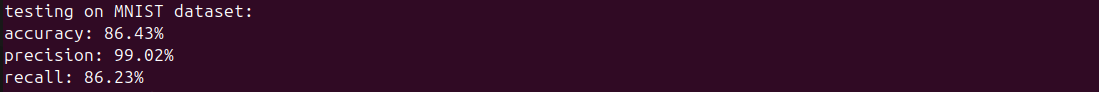
\includegraphics[width=1\textwidth]{images/tree_mnist_test_stats.png}
	\caption{Statystyki: accuracy, precision, recall, loss, w teście Random Tree na zbiorze EMNIST MNIST}
\end{figure}

\begin{figure}[h!]
	\centering
	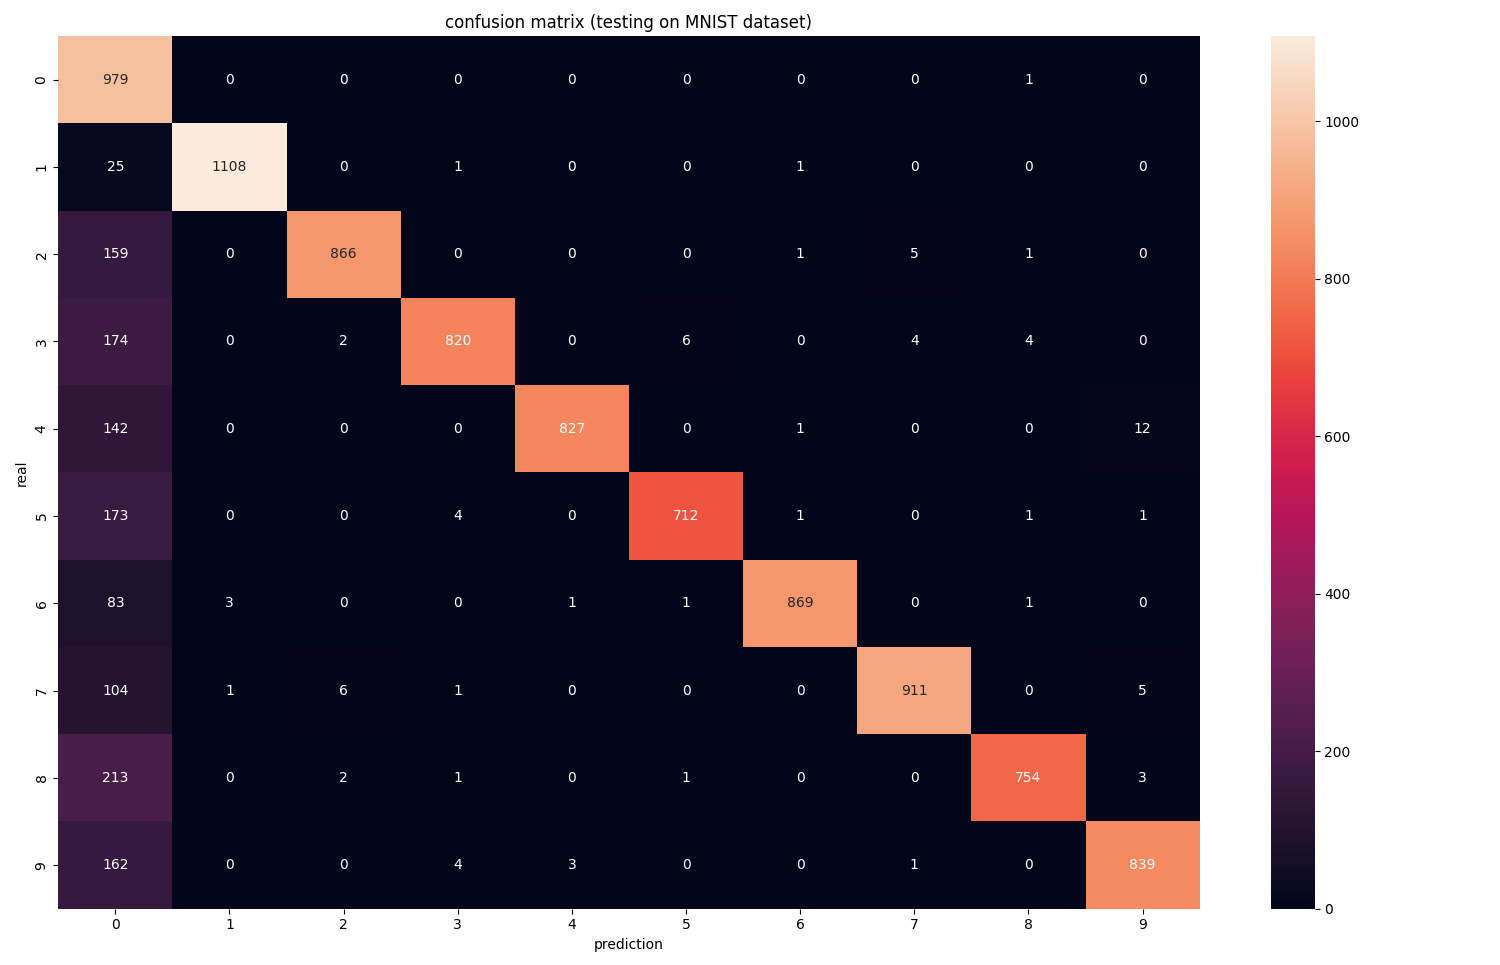
\includegraphics[width=1\textwidth]{images/tree_mnist_conf_matrix.png}
	\caption{Confusion matrix dla testów Random Tree na zbiorze EMNIST MNIST}
\end{figure}

\section*{Testy Random Tree na własnym zbiorze testowym}
\begin{lstlisting}[language=Python, frame=single, breaklines=true, breakatwhitespace=true]
# testowanie na własnym zbiorze
print("testing on my dataset:")
y_pred_prob = model.predict(x_my)

acc = accuracy_score(y_my, y_pred_prob)
precision = precision_score(y_my, y_pred_prob, average='macro')
recall = recall_score(y_my, y_pred_prob, average='macro')

print(f"accuracy: {acc*100:.2f}%")
print(f"precision: {precision*100:.2f}%")
print(f"recall: {recall*100:.2f}%")

y_pred = np.argmax(y_pred_prob, axis=1)
y_real = np.argmax(y_my, axis=1)
conf_matrix = confusion_matrix(y_real, y_pred)

fig, ax = plt.subplots(figsize=(15, 10))
ax = sb.heatmap(conf_matrix, annot=True, fmt='d', ax=ax)
ax.set_xlabel('prediction')
ax.set_ylabel('real')
ax.set_title('confusion matrix (testing on my dataset)')

plt.tight_layout()
plt.show()
\end{lstlisting}

\begin{figure}[h!]
	\centering
	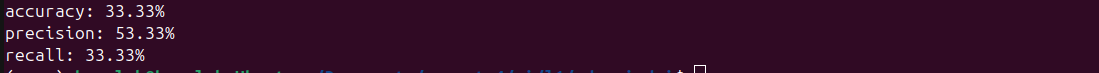
\includegraphics[width=1\textwidth]{images/tree_my_test_stats.png}
	\caption{Statystyki: accuracy, precision, recall, loss, w teście Random Tree na moim zbiorze}
\end{figure}

\begin{figure}[h!]
	\centering
	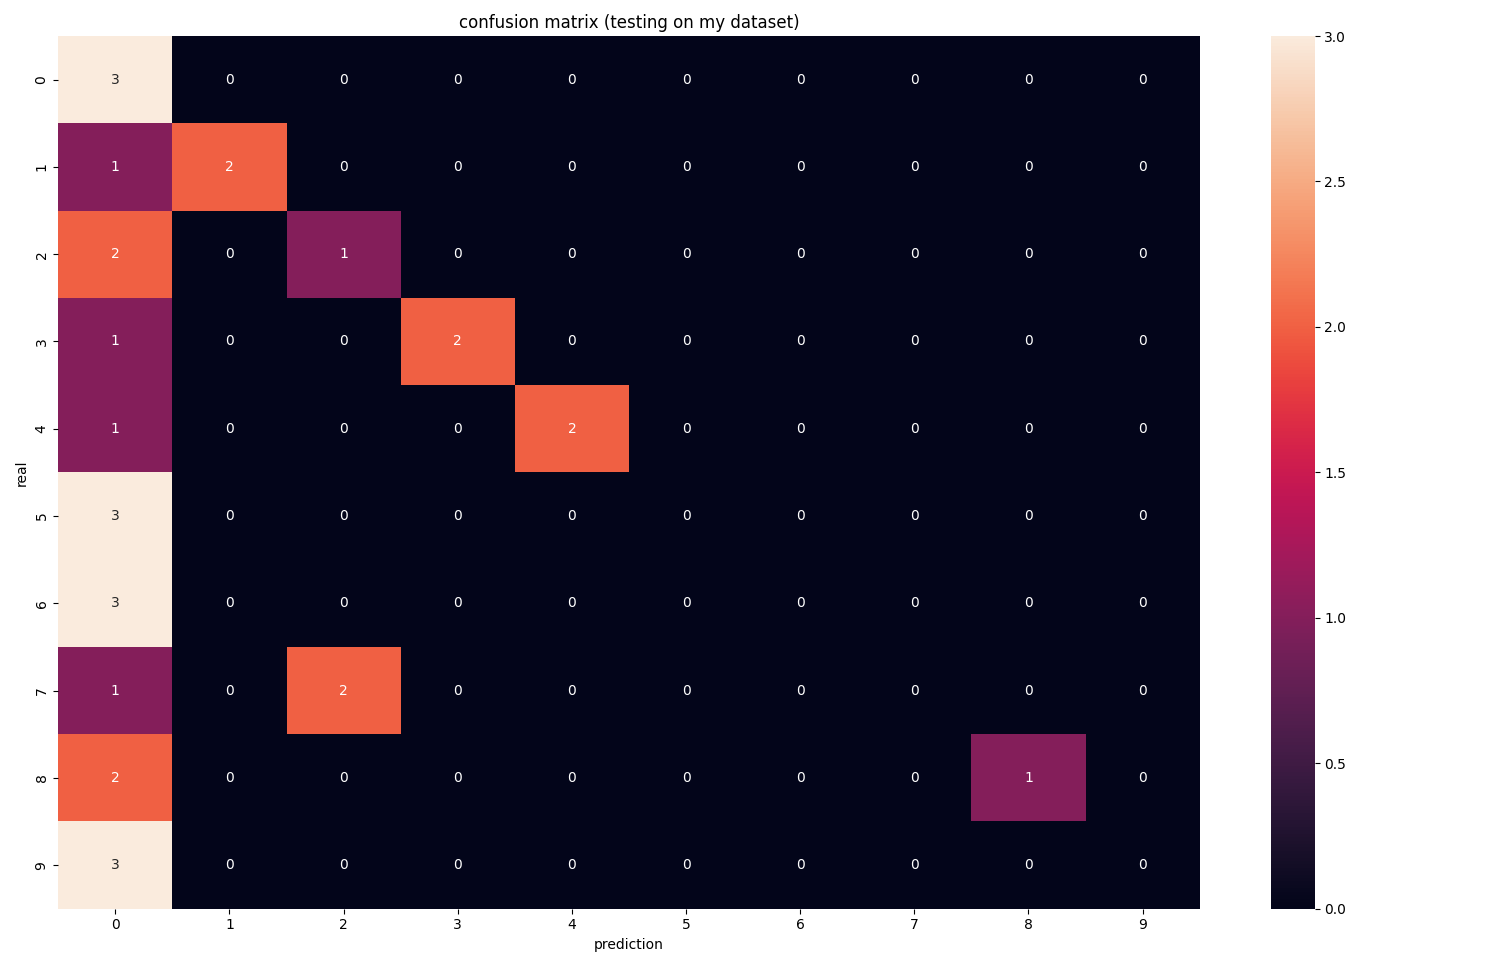
\includegraphics[width=1\textwidth]{images/tree_my_conf_matrix.png}
	\caption{Confusion matrix dla testów Random Tree na moim zbiorze}
\end{figure}

\end{document}
